%Linea Para poder completar automaticamente las citas con el Sublime
%No hace el documento, se puede borrar esta linea si no se usa el Sublime
%------------------------------------------------------------------------------
 \newcommand{\NoBiblioBT}[1]{
 \ifthenelse{\equal{#1}{verdadero}}{}{\bibliography{Referencias/base_bibliografica}}
 \NoBiblioBT{verdadero}}
 %-----------------------------------------------------------------------------
 
%Formato (Nombre de capitulo largo o corto), nombre del capitulo y estilo de la
%Portada del Capitulo
%------------------------------------------------------------------------------

 %Formato en si, titulo en un solo renglon
 \FormatoCapituloDosLineas
 
 %Nombre y etiquete para referir
 \chapter{Tratamientos alternativos de síntesis a bajas temperaturas}
 \label{chap:Optimizacion}

 %Para que no salga el numero de pagina en la portada del capitulo
 \thispagestyle{empty}
	
 %Resumen del Capitulo en Italica
 \noindent\textit{En este capítulo se analizaron los resultados de los métodos desarrollados para sintetizar películas mesoporosas por debajo de \SI{130}{\celsius}. Ya se expuso, anteriormente, el dominio adquirido sobre la química de los materiales, reacciones sol-gel y técnicas de depósito. También se demostró la accesibilidad de los poros, accesibilidad al electrodo y adherencia sobre distintos sustratos. Con estos conocimientos, la siguiente etapa, consistió en desarrollar películas de SiO$_2$ a bajas temperaturas, de forma de evitar tratamientos de calcinación. Los métodos suaves, a bajas temperaturas, permiten una mayor compatibilidad de procesos\textit{ top-down} y\textit{ bottom-up}, bajar costos en la síntesis y abrir la posibilidad de depositar las películas sobre sustratos en materiales poliméricos, flexibles y de bajo costo.}\label{reemplazo1}
 
 %Indice de capitulo alineada al borde inferior de la pagina, nueva pagina
 \vfill
 \minitoc
 \newpage
 %-------------------------------------------------------------------------------

\section{Introducción}

	Uno de los objetivos principales que tiene este trabajo de tesis es compatibilizar los procesos \textit{bottom-up}, utilizados en la síntesis de las películas delgadas mesoporososas, y los procesos \textit{top-down}, los cuales son necesarios para fabricar los sensores. Otro, es flexibilizar los procesos de síntesis y microfabricación, para poder incluir cada vez, materiales más diversos y, a su vez, poder tener mayores opciones a la hora de elegir de que forma fabricar los sensores para aplicaciones dedicadas\cite{Doshi2000a,Wagner2013,Innocenzi2013,Soler-Illia2002a}.

	Para ir en la dirección de concretar ambos objetivos se exploró la posibilidad de sintetizar las películas delgadas mesoporosas bajando la temperatura durante el proceso de síntesis. Recordemos que la misma involucra un paso de calcinación a \SI{350}{\celsius}, que promueve la condensación del óxido y, a su vez, calcina el surfactante (materia orgánica) dando lugar a la formación de los poros.\cite{Zhang2015,Horiuchi2011,Clark2000,Zhang2005}

	La búsqueda de métodos de síntesis a bajas temperaturas permitiría fabricar los electrodos con Au metalúrgico o carbono (ver capitulo \ref{chap:Microfabricacion}, donde se desarrolla en profundidad estos aspectos) e incorporar sustratos poliméricos, como acrílico, resinas de poliéster, polibutileno de tereftalato (PBT), polietileno de tereftalato (PET), abriendo la posibilidad de utlizar una gama de materiales mucho mas amplia y abaratando costos.

\section{Tratamientos alternativos a bajas temperaturas}
	
		En función de lo expuesto anteriormente se experimentaron cinco procesos alternativos a la calcinación. Unos basados en condensación a bajas temperaturas durante distintos tiempos, otros basados en catálisis química y un último basado en desplazamiento del equilibrio químico. Al omitir el proceso de calcinación se realizó sobre todos ellos una etapa de extracción y lavado para remover el surfactante de la estructura porosa. Los detalles experimentales fueron descritos en la sección \ref{sec:cond_y_extr}, pág \pageref{sec:cond_y_extr}.

		Se realizó un trabajo sistemático de caracterización, para cada tratamiento, para películas mesoestructuradas con F127 y con CTAB (denominadas \pdmF\space y \pdmC\space respectivamente). Se empleó elipsoporosimetría ambiental (PEA) para caracterizar espesor, tamaño de poro y cuellos; FTIR para análisis de la condensación siguiendo la evolución de la forma de la banda LO$_3$ y la relación de los picos correspondientes a las vibraciones Si-O-Si y Si-OH (ver la sección \ref{sec:IR}, pág. \pageref{sec:IR}, para un análisis detallado de los espectros IR); y microcopías ópticas y electrónicas para evaluar morfología, adherencia e integridad de las películas.

	\subsection{Tratamiento simplificado}

		De todos los tratamientos post-deposito, este fue el más sencillo de todos. Consintió simplemente en extrae el surfactante luego de tratar la muestra a \SI{130}{\celsius} durante \SI{1}{\hour}. La extracción se llevó a cabo con un reflujo de 2-propanol durante 15 min. 
		
		En el análisis por microscopía óptica para \pdmF\space (figura \ref{fig:Microscopia_F127_simplificado}) se aprecia que las película sintetizadas con este tratamiento se adhieren bien y quedan bien formadas, sin grietas ni discontinuidades, tanto sobre Au como sobre Si. También se observa en el recuadro de las figuras  la presencia de poros bien formados sobre la superficie para ambos sustratos.
			
			\begin{figure}[th]
		 	   	    \begin{subfigure}[t]{0.49\textwidth}
			       	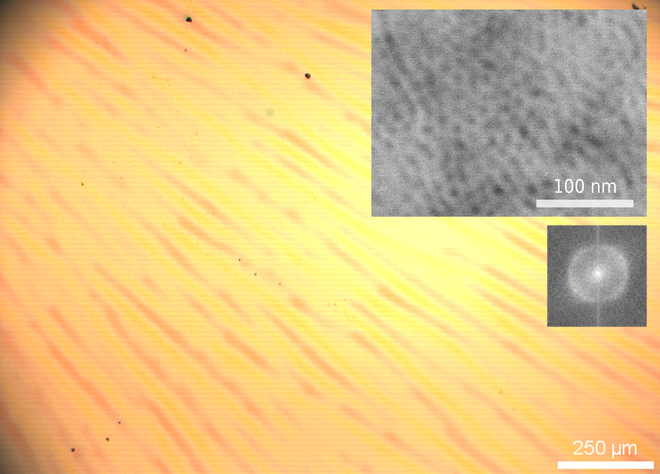
\includegraphics[width=\textwidth]{Imagenes/Au_EtF127-Combinada.jpg}
			   		\end{subfigure}
			   		\begin{subfigure}[t]{0.49\textwidth}
			   	    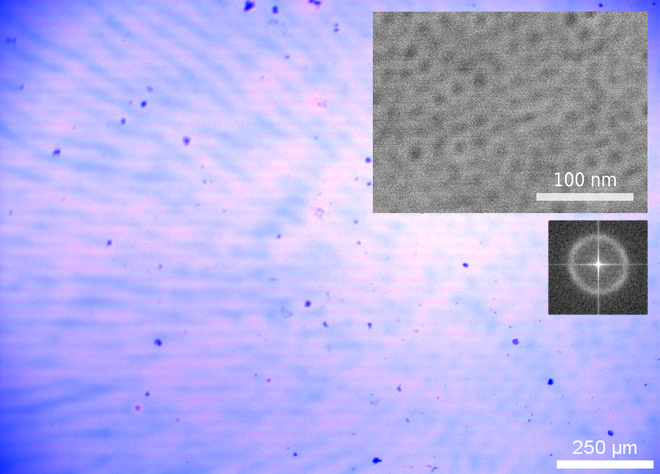
\includegraphics[width=\textwidth]{Imagenes/Si_EtF127-Combinada.jpg}
			   		\end{subfigure}
					 \caption[Microscopías \pdmF\space tratamiento simplificado.]{Microscopías ópticas para \pdmF\space sintetizadas por el tratamiento simplificado. Izquierda: sobre sustrato de Au. Derecha: sobre sustrato de Si. En los respectivos recuadros se observa el detalle por MEB del arreglo nanoporoso.}
					 \label{fig:Microscopia_F127_simplificado}	
				     \end{figure}		

		En la figura \ref{fig:F127_simplificado_EPA} se presentan las mediciones por PEA para las \pdmF. Allí se observa que las desorción de agua ocurre en dos etapas, a dos humedades relativas (P/P$_s$) diferentes, en $0,65$ y en $0,45$. En los trabajos de Jörg P. Thielemann \cite{Thielemann2011} y Johan C. Groen\cite{Groen2003} se propone que este comportamiento, de la desorción en dos etapas, se produce al desorber el agua ocluida en poros que están más o menos <<bloqueados>> por el diámetro de los cuellos. Al producirse la desorción del agua a través de cuellos de distintos tamaño, la fuerza  necesaria para vencer la tensión superficial debe ser mayor, desorbiendo a menores P/P$s$ cuanto menores sea el diámetro de los cuellos; tal como predice la ecuación de Kelvin (ver ecuación {\ref{eq:kelvin}). Esta doble distribución de tamaño de cuellos también se ve reflejada en el gráfico de la figura \ref{fig:F127_simplificado_PSD} donde se gráfican las distribuciones de tamaño de poro y cuello.

			\begin{figure}[th]
			  	\begin{subfigure}[t]{0.495\textwidth}
			  	\includegraphics[width=\textwidth]{Graficos/SI_F127_simplificado_EPA.pdf}
				\caption{Isorterma de adsorción/desorción de agua realizada por PEA para una \pdmF.}
				\label{fig:F127_simplificado_EPA}
				\end{subfigure}
				\begin{subfigure}[t]{0.495\textwidth}
			  	\includegraphics[width=\textwidth]{Graficos/SI_F127_simplificado_PSD.pdf}
				\caption{Distribución de tamaño de poro y cuello.\\ }
				\label{fig:F127_simplificado_PSD}
				\end{subfigure}
				\caption[Elipsoporosimetría \pdmF\space tratamiento simplificado.]{Resultados de elipsoporosimetría ambiental para una \pdmF\space sintetizada por el tratamientos simplificado.}
				\label{fig:F127_simplificado}
				\end{figure}

			\begin{figure}[ht]
				\begin{center}
				\includegraphics[width=0.75\textwidth]{Graficos/IR_F127_simplificado.pdf}
				\caption[FTIR \pdmF\space tratamiento simplificado.]{Espectro de absorción en el IR para una \pdmF\space sintetizada con el tratamiento simplificado antes y después de extraer el surfactante. Desaparece la banda de estiramiento C-H correspondiente al surfactante luego de la extarcción.}
				\label{fig:IR_F127_simplificado}
				\end{center}
				\end{figure}

		En la figuras \ref{fig:IR_F127_simplificado} se comparan el espectro de absorción en el IR para una \pdmF\space antes y después de practicar la extracción del surfactante. Se ve como desaparece el pico correspondiente al surfactante (estiramiento C-H) luego de la extracción. También se observa la típica banda de la vibración TO$_3$ de silice mesoporosa en $\approx \text{\SI{1070}{\cm^{-1}}}$.

		En el caso del tratamiento simplificado, cuando las películas mesoporosas son estructuradas con CTAB, se observan que estám bien formadas sobre silicio pero no sobre Au (figura \ref{fig:Microscopia_CTAB_simplificado}). Allí la estructura presenta grietas y discontinuidades, posiblemente se deba al hecho de la adsorción del bromuro sobre el Au, ya discutido en la sección \ref{sec:adherencia}, pág. \pageref{sec:adherencia}.

			\begin{figure}[th]
		 	   	    \begin{subfigure}[t]{0.49\textwidth}
			       	\includegraphics[width=\textwidth]{Imagenes/Au_EtCTAB-Combinada.jpg}
			   		\end{subfigure}
			   		\begin{subfigure}[t]{0.49\textwidth}
			   	    \includegraphics[width=\textwidth]{Imagenes/Si_EtCTAB-Combinada.jpg}
			   		\end{subfigure}
					 \caption[Microscopías \pdmC\space tratamiento simplificado.]{Microscopías ópticas para \pdmC\space sintetizadas por el tratamiento simplificado. Observese las grietas presentes cuando se sintetiza sobre Au (izquierda), mientras que sobre Si las \pdmC\space no presentan rupturas ni discontinuidades.}
					 \label{fig:Microscopia_CTAB_simplificado}	
				     \end{figure}	
		
		En la figura \ref{fig:CTAB_simplificado_EPA} se muestra la medición por PEA para las \pdmC\space sintetizadas por el mismo tratamiento. Se ve que que la porosidad es alta, aproximadamente 40\%, sin embargo la isoterma no presenta casi histéresis entre las ramas de adsorción y desorción. Esto significa, que no hay prácticamente diferencia entre el tamaño de poro y cuello, como se muestra en la figura \ref{fig:CTAB_simplificado_PSD} donde se gráfica la distribución de cuellos y poros. Este tamaño pequeño en el diámetro de poro se puede atribuir a un residuo de surfactante en la estructura, en el IR (figura \ref{fig:IR_CTAB_simplificado}) se ve dicho residuo en el espectro correspondiente a la película extraída con 2-pronanol. El hecho de exista esa cantidad de residuo remanente, se lo atribuye a la baja condensación que presentan las películas con este tratamiento, ya que de queda surfactante retenido en la red de silice parcialmente condensada.

		\begin{figure}[!ht]	
			\begin{subfigure}[t]{0.495\textwidth}
		  	\includegraphics[width=\textwidth]{Graficos/SI_CTAB_simplificado_EPA.pdf}
			\caption{Isorterma de adosroción/desorción de agua ralizada por PEA para una \pdmC.}
			\label{fig:CTAB_simplificado_EPA}
			\end{subfigure}
			\begin{subfigure}[t]{0.495\textwidth}
		  	\includegraphics[width=\textwidth]{Graficos/SI_CTAB_simplificado_PSD.pdf}
			\caption{Distribución de tamaño de poro y cuello.\\ }
			\label{fig:CTAB_simplificado_PSD}
			\end{subfigure}
			\caption[Elipsoporosimetría \pdmC\space tratamiento simplificado.]{Resultados de elipsoporosimetría ambiental para una \pdmC\space sintetizada por el tratamientos simplificado.}
			\end{figure}
		
		\begin{figure}[!ht]
			\begin{center}
			\includegraphics[width=0.75\textwidth]{Graficos/IR_CTAB_simplificado.pdf}
			\caption[FTIR \pdmC\space tratamiento simplificado.]{Espectro de absorción en el IR para una \pdmC\space sintetizada con el tratamiento simplificado antes y después de extraer el surfactante. Todavía se puede apreciar un cantidad pequeña de surfactante luego de la extracción.}
			\label{fig:IR_CTAB_simplificado}
			\end{center}
			\end{figure}	

	\subsection{Tratamiento prolongado}

		Otro de los tratamientos que se experimentó fue el de realizar una condensación a \SI{130}{\celsius} durante un período de 7 días. 

		Para el F127 se logró sintetizar películas homogéneas sin discontinuidades, tanto para sustratos de Au como para sustratos de Si. Al igual que en el caso anterior, en la figura \ref{fig:Microscopia_F127_prolongado}, se muestran estos resultados, y, en los respectivos recuadros, se observa nuevamente los nanoporoso, donde, antes de la extracción, se ubicaban las miscelas de F127. 

		 \begin{figure}[th]
		 	   	    \begin{subfigure}[t]{0.49\textwidth}
			       	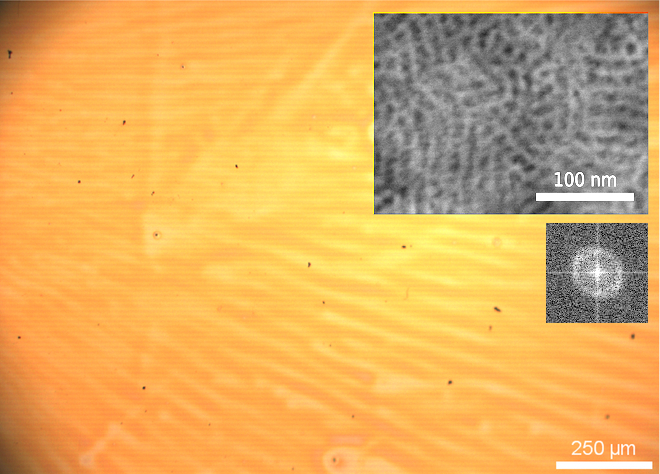
\includegraphics[width=\textwidth]{Imagenes/Au_130F127-Combinada.jpg}
			   		\end{subfigure}
			   		\begin{subfigure}[t]{0.49\textwidth}
			   	    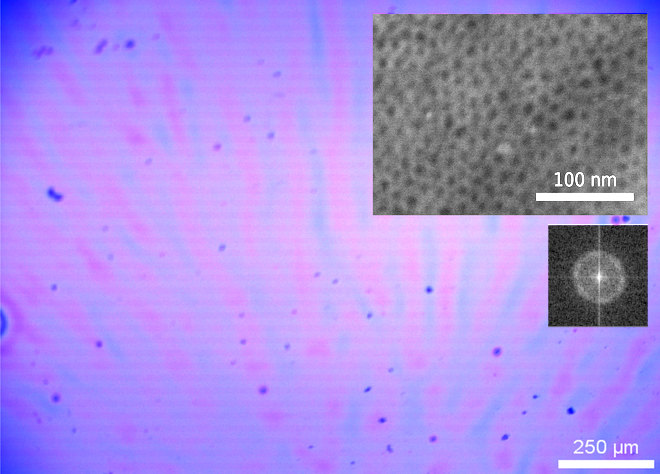
\includegraphics[width=\textwidth]{Imagenes/Si_130F127-Combinada.jpg}
			   		\end{subfigure}
					 \caption[Microscopía \pdmF tratamiento prolongado.]{Microscopías ópticas para \pdmF\space sintetizadas por el tratamiento prolongado. Izquierda: sobre sustrato de Au. Derecha: sobre sustrato de Si. En los respectivos recuadros se observa el detalle por MEB del arreglo nanoporoso.}
					 \label{fig:Microscopia_F127_prolongado}	
				     \end{figure}	
		
		Respecto de la caracterización por PEA, para el F127, se observa la misma distribución de <<doble cuello>> o poros bloqueados que en el caso del tratamiento simplificado (figura \ref{fig:F127_prolongado_EPA}). 

		 \begin{figure}[!ht]
			  	\begin{subfigure}[t]{0.495\textwidth}
			  	\includegraphics[width=\textwidth]{Graficos/SI_F127_prolongado_EPA.pdf}
				\caption{Isorterma de adosroción/desorción de agua ralizada por PEA para \pdmF.}
				\label{fig:F127_prolongado_EPA}
				\end{subfigure}
				\begin{subfigure}[t]{0.495\textwidth}
			  	\includegraphics[width=\textwidth]{Graficos/SI_F127_prolongado_PSD.pdf}
				\caption{Distribución de tamaño de poro y cuello.\\ }
				\label{fig:F127_prolongado_PSD}
				\end{subfigure}
				\caption[Elipsoporosimetría \pdmF\space tratamiento prolongado.]{Resultados de elipsoporosimetría ambiental para una \pdmF\space sintetizada por el tratamientos prolongado, 7 días a \SI{130}{\celsius} luego de la estabilización del deposito.}
		 		\end{figure}

		En el caso del CTAB se logró sintetizar películas delgadas homogéneas y sin fisuras solo para el silicio, tal como 
		se muestra en la microscopía de la figura \ref{fig:Microscopia_CTAB_prolongado}. 

		Cuando se depositaron sobre sustrato de Au, se vuelven a observar grietas y sectores enteros <<despegados>>. En el recuadro de la figura \ref{fig:Microscopia_CTAB_prolongado} se observa el detalle de algunas de estas discontinuidades en las películas. 		
		 \begin{figure}[!th]
	 	   	    \begin{subfigure}[t]{0.49\textwidth}
		       	\includegraphics[width=\textwidth]{Imagenes/Au_130CTAB-Combinada.jpg}
		   		\end{subfigure}
		   		\begin{subfigure}[t]{0.49\textwidth}
		   	    \includegraphics[width=\textwidth]{Imagenes/Si_130CTAB-Combinada.jpg}
		   		\end{subfigure}
				 \caption[Microscopía óptica \pdmC\space tratamiento prolongado.]{Microscopías ópticas para \pdmC\space sintetizadas por el tratamiento prolongado. Derecha: sobre sustrato de Au. Izquierda: sobre sustrato de Si.}
				 \label{fig:Microscopia_CTAB_prolongado}	
			     \end{figure}	
			     
		Las elipsoporosimetrías para este sistema, es decir, poros formados por miscelas de CTAB y sintetizados por el tratamiento prolongado, muestra isotermas prácticamente idénticas al sistema calcinado, con poros de \SI{2,5}{nm} y cuellos de \SI{1,9}{nm}.
			     
		 \begin{figure}[!ht]
		  	\begin{subfigure}[t]{0.495\textwidth}
		  	\includegraphics[width=\textwidth]{Graficos/SI_CTAB_prolongado_EPA.pdf}
			\caption{Isoterma de adosroción/desorción de agua ralizada por PEA para \pdmC\space.}
			\label{fig:CTAB_prolongado_EPA}
			\end{subfigure}
			\begin{subfigure}[t]{0.495\textwidth}
		  	\includegraphics[width=\textwidth]{Graficos/SI_CTAB_prolongado_PSD.pdf}
			\caption{Distribución de tamaño de poro y cuello.\\ }
			\label{fig:CTAB_prolongado_PSD}
			\end{subfigure}
			\caption[Elipsoporosimetría \pdmC\space tratamiento prolongado.]{Resultados de elipsoporosimetría ambiental para una \pdmC\space sintetizada por el tratamientos prolongado, 7 días a \SI{130}{\celsius} luego de la estabilización del deposito.}
			\end{figure}

		Los gráficos de espectroscopia IR para ambos sistemas de poros, F127 y CTAB (figuras \ref{fig:IR_F127_prolongado} y \ref{fig:IR_CTAB_prolongado}),  muestran que la extracción fue exitosa. Si bien en caso de las \pdmC\space se ve todavía una pequeña cantidad de surfactante, la cantidad relativa al no extraído es mucho menor que en el tratamiento simplificado, indicando que la extracción fue mejor. %Poner referencias aca!!!!!!
		
		\begin{figure}[!ht]
			\begin{center}
			\includegraphics[width=0.75\textwidth]{Graficos/IR_F127_prolongado.pdf}
			\caption[FTIR \pdmF\space tratamiento prolongado.]{Espectro de absorción de IR correspondiente a una \pdmF\space sintetizada por el tratamiento prolongado antes y después de la extracción con 2-propanol.}
			\label{fig:IR_F127_prolongado}
			\end{center}
			\end{figure}
		
		\begin{figure}[!ht]
			\begin{center}
			\includegraphics[width=0.75\textwidth]{Graficos/IR_CTAB_prolongado.pdf}
			\caption[FTIR \pdmC\space tratamiento prolongado.]{Espectro de absorción de IR correspondiente a una \pdmC\space sintetizada por el tratamiento prolongado antes y después de la extracción con 2-propanol.}
			\label{fig:IR_CTAB_prolongado}
			\end{center}
			\end{figure}	

		\pagebreak

	\subsection{Tratamiento alto vacío}\label{sec:trat-vacio}
	
		Luego del éxito parcial tratamiento prolongado, donde se obtuvieron películas homogéneas y con arreglos de poros bien formados, con estructuras comparables con los mesoporoso calcinado\cite{Mogilnikov2002,Fuertes2008,Rothen1945}, se hizo un tratamiento similar, en cuanto a tiempo y temperatura (7 días a \SI{130}{\celsius}), pero colocando las muestras en alto vacío (ver sección \ref{sec:cond_y_extr}, pág. \pageref{sec:cond_y_extr}).

		El motivo de llevar a cabo este tratamiento fue abastecer al sistema de calor, durante un cierto tiempo, para darle oportunidad de relajar y estabilizar el cristal líquido y, a la vez, aplicando vacío, desplazar el equilibrio de la reacción  \ref{eq:vacio} según el principio de Le Chatelier\cite{Atkins2006}, removiendo productos de reacción volátiles (H$_2$O y alcoholes) y así favorecer la condensación del óxido.\cite{Zhuravlev2000}

		\begin{equation}
				 \schemestart 
				 Si-OH + X-O-Si 
				 \arrow{->[\scriptsize{T=\SI{130}{\celsius},P=\SI{1e-5}{\milli\bar}}][\scriptsize{X=H,CH$_3$CH$_2$}]}[0,2.5] 
				 Si-O-Si + X-OH $\hspace{-0.1cm}\Big\uparrow$
				 \schemestop
				 \label{eq:vacio}
				 \end{equation}

		\begin{figure}[!th]
	 	   	    \begin{subfigure}[t]{0.49\textwidth}
		       	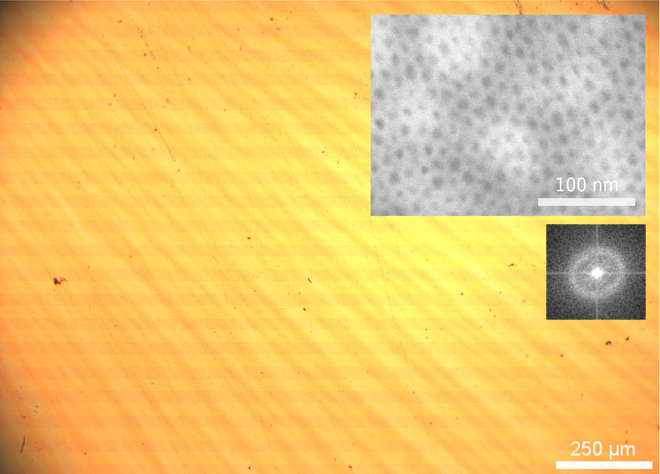
\includegraphics[width=\textwidth]{Imagenes/Au_130VF127-Combinada.jpg}
		   		\end{subfigure}
		   		\begin{subfigure}[t]{0.49\textwidth}
		   	    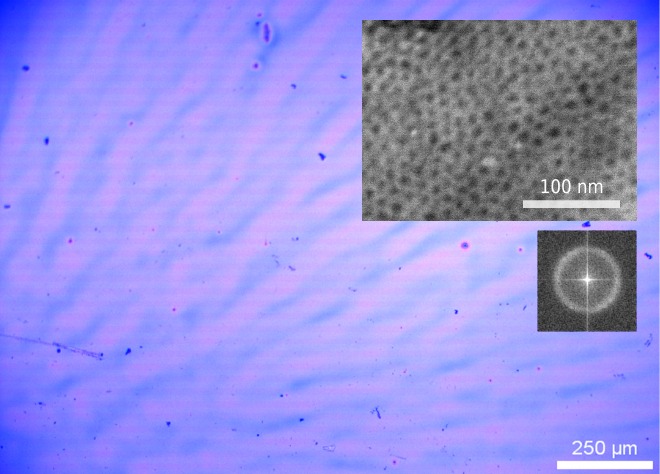
\includegraphics[width=\textwidth]{Imagenes/Si_130VF127-Combinada.jpg}
		   		\end{subfigure}
				 \caption[Microscopía óptica \pdmF\space tratamiento vacío.]{Microscopías ópticas para \pdmF\space sintetizadas por el tratamiento de condensación y extracción por alto vacío. Izquierda: sobre sustrato de Au. Derecha: sobre sustrato de Si. En los respectivos recuadros se observa el detalle por MEB del arreglo nanoporoso.}
				 \label{fig:Microscopia_F127_vacio}	
			     \end{figure}	

		\pagebreak

		Las microscopías ópticas muestran películas homogéneas, sin discontinuidades ni grietas. Las microscopías electrónicas revelan la presencia de nanoporos sobre ambos sustratos, silicio y oro (ver figura \ref{fig:Microscopia_F127_vacio}) 

		En las mediciones por PEA, para el caso del F127 (figuras \ref{fig:F127_vacio_EPA} y \ref{fig:F127_vacio_PSD}), desaparece la <<doble distribución>> de cuellos,  mostrando una isoterma que alcanza un índice de refracción de $n=1,25$ (a HR=0\%) y una porosidad de $30\%$, valores próximos a los esperados para un sistema calcinado.

		\begin{figure}[!ht]
			  	\begin{subfigure}[t]{0.495\textwidth}
			  	\includegraphics[width=\textwidth]{Graficos/SI_F127_vacio_EPA.pdf}
				\caption{Elipsoporosimetría de una \pdmF\space tratamiento 7 días en alto vacío.}
				\label{fig:F127_vacio_EPA}
				\end{subfigure}
				\begin{subfigure}[t]{0.495\textwidth}
			  	\includegraphics[width=\textwidth]{Graficos/SI_F127_vacio_PSD.pdf}
				\caption{Distribución de tamaño de poro y cuello.\\ }
				\label{fig:F127_vacio_PSD}
				\end{subfigure}
				\caption[Elipsoporosimetría \pdmF\space tratamiento alto vacío.]{Resultados de elipsoporosimetría ambiental para una \pdmF\space sintetizada por el tratamientos prolongado, 7 días a \SI{130}{\celsius} en alto vacío (P=\SI{1e-5}{\milli\bar}).}
				\end{figure}

		Respecto de las películas estructuradas con CTAB, presenta el mismo comportamiento que en los caso anteriores, se observa un deposito homogéneo y sin grietas cuando se depositan sobre silicio, pero se observan discontinuidades y grietas cuando se depositan sobre Au, tal como se muestra en la figura \ref{fig:Microscopia_CTAB_vacio}.
		
		\begin{figure}[!th]
		 	   	    \begin{subfigure}[t]{0.49\textwidth}
			       	\includegraphics[width=\textwidth]{Imagenes/Au_130VCTAB-Combinada.jpg}
			   		\end{subfigure}
			   		\begin{subfigure}[t]{0.49\textwidth}
			   	    \includegraphics[width=\textwidth]{Imagenes/Si_130VCTAB-Combinada.jpg}
			   		\end{subfigure}
					 \caption[Microscopía óptica \pdmC tratamiento vacío.]{Microscopías ópticas para \pdmC\space sintetizadas por el tratamiento en alto vacío. Izquierda: sobre sustrato de Au. Derecha: sobre sustrato de Si.}
					 \label{fig:Microscopia_CTAB_vacio}	
				     \end{figure}		     

		La isoterma por PEA para este sistema presenta una porosidad alta y un índice de refracción prácticamente igual al del calcinado (figura \ref{fig:CTAB_vacio_EPA}) y la distribución de tamaño de poros que se muestra en la figura \ref{fig:CTAB_vacio_PSD} y cuellos es comparable con la reportada en literatura \cite{Boissiere2005}

		\pagebreak		     
				     
 		\begin{figure}[!ht]
		  	\begin{subfigure}[t]{0.495\textwidth}
		  	\includegraphics[width=\textwidth]{Graficos/SI_CTAB_vacio_EPA.pdf}
			\caption{Elipsoporsimetría de una \pdmC\space Tratamiento 7 días alto vacío.}
			\label{fig:CTAB_vacio_EPA}
			\end{subfigure}
			\begin{subfigure}[t]{0.495\textwidth}
		  	\includegraphics[width=\textwidth]{Graficos/SI_CTAB_vacio_PSD.pdf}
			\caption{Distribución de tamaño de poro y cuello.\\ }
			\label{fig:CTAB_vacio_PSD}
			\end{subfigure}
			\caption[Elipsoporosimetría \pdmC\space tratamiento alto vacío.]{Resultados de elipsoporosimetría ambiental para una \pdmC\space sintetizada por el tratamientos prolongado, 7 días a \SI{130}{\celsius} en alto vacío (P=\SI{1e-5}{\milli\bar}).}
			\end{figure} 	
		
		La extracción del surfactante (ya sea para las películas estructuradas con F127 o estructuradas con CTAB), se llevó a cabo de la misma forma que que en los caso anteriores; sometiendo a las películas a un reflujo de 2-propanol durante \SI{15}{\minute}. 

		Los espectros de absorción IR se muestran en las figuras \ref{fig:IR_F127_vacio} y \ref{fig:IR_CTAB_vacio} para F127 y CTAB respectivamente.		

		\begin{figure}[!ht]
			 	\begin{center}
			 	\includegraphics[width=0.75\textwidth]{Graficos/IR_F127_vacio.pdf}
			 	\caption[FTIR \pdmF\space tratamiento prolongado.]{Espectro de absorción de IR correspondiente a una \pdmF\space sintetizada por el tratamiento prolongado en alto vacío, antes y después de la extracción con 2-propanol.}
			 	\label{fig:IR_F127_vacio}
			 	\end{center}
			 	\end{figure}
			
		\pagebreak
					
		\begin{figure}[!ht]
			 	\begin{center}
			 	\includegraphics[width=0.75\textwidth]{Graficos/IR_CTAB_vacio.pdf}
			 	\caption[FTIR \pdmC\space tratamiento prolongado.]{Espectro de absorción de IR correspondiente a una \pdmC\space sintetizada por el tratamiento prolongado en alto vacío, antes y después de la extracción con 2-propanol.}
			 	\label{fig:IR_CTAB_vacio}
			 	\end{center}
			 	\end{figure}
			
	\subsection{Tratamiento ácido}
		
		Algunos autores proponen que un medio fuertemente ácido (pH$<1$) favorece la hidrólisis del alcóxido y la condensación de los grupo siloxano \cite{Soler-Illia2011,Doshi2000a,Boissiere2000,Huo1996,Beck1992}. Las películas depositadas, estabilizadas en cámara de humedad y  parcialmente condensadas a \SI{130}{\celsius}, tal como se explica en la sección \ref{sec:cond_y_extr}, pág. \pageref{sec:cond_y_extr}, fueron expuestos a una atmósfera de HCl durante \SI{15}{\minute}. 

		En la figura \ref{fig:Microscopia_F127_acido} se presentas las microscopias ópticas para películas estructuras con F127 sintetizadas por el método de atmósfera ácida. Se observan grietas en las películas depositadas sobre películas delgadas de Au, debido a una condensación rápida catalizada por el medio ácido. Al no tener una excelente adherencia sobre el sustrato, se contraen en todas las direcciones y no solo en la dirección normal a la superficie, como es en el caso del silicio\cite{Sakatani2006,Boissiere2005,Guillemin2010}. En ese caso las películas quedan bien formadas. Sin embargo, en por microscopía electrónica (recuadro figura \ref{fig:Microscopia_F127_acido}) se observan los poros casi unidos formando una especie de poro elongado.

		\begin{figure}[!th]
	 	   	    \begin{subfigure}[t]{0.49\textwidth}
		       	\includegraphics[width=\textwidth]{Imagenes/Au_AF127-Combinada.jpg}
		   		\end{subfigure}
		   		\begin{subfigure}[t]{0.49\textwidth}
		   	    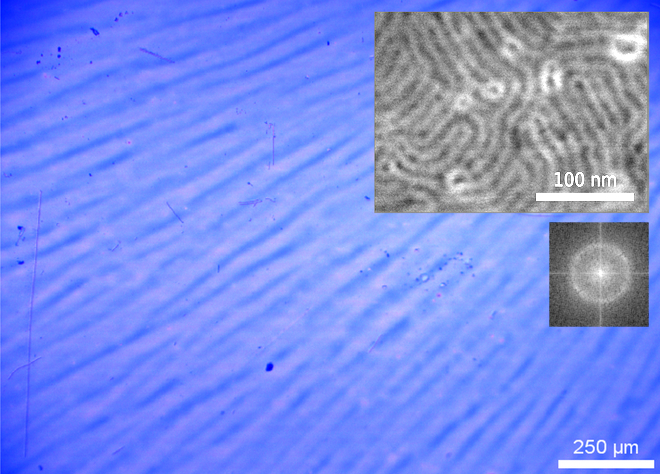
\includegraphics[width=\textwidth]{Imagenes/Si_AF127-Combinada.jpg}
		   		\end{subfigure}
				 \caption[Microscopía óptica \pdmF tratamiento en medio ácido.]{Microscopías ópticas para \pdmF\space sintetizadas por el tratamiento de condensación y extracción en medio ácido. Izquierda: sobre sustrato de Au. Derecha: sobre sustrato de Si. En los respectivos recuadros se observa el detalle por MEB del arreglo nanoporoso.}
				 \label{fig:Microscopia_F127_acido}	
			     \end{figure}	

		Esta morfología superficial de los poros se corrobora con el gráfico de la figura \ref{fig:F127_acido_EPA}, donde se observa en la isoterma de adsorción/desorción de agua una <<doble distribución>> de cuellos, sin embargo, en este caso predominan los cuellos de diámetro pequeño, siendo los grandes casi del mismo tamaño que los poros, como se ve por microscopía electrónica de la figura \ref{fig:Microscopia_F127_acido}.
		
		\begin{figure}[!ht]
		  	\begin{subfigure}[t]{0.495\textwidth}
		  	\includegraphics[width=\textwidth]{Graficos/SI_F127_acido_EPA.pdf}
			\caption{Isoterma de adsorción/desorción de agua realizada por PEA para una \pdmF.}
			\label{fig:F127_acido_EPA}
			\end{subfigure}
			\begin{subfigure}[t]{0.495\textwidth}
		  	\includegraphics[width=\textwidth]{Graficos/SI_F127_acido_PSD.pdf}
			\caption{Distribución de tamaño de poro y cuello.\\ }
			\label{fig:F127_acido_PSD}
			\end{subfigure}
			\caption[Elipsoporosimetría \pdmF\space tratamiento ácido.]{Resultados de elipsoporosimetría ambiental para una \pdmF\space sintetizada por el tratamiento en medio ácido.}
			\end{figure}

		Las películas nanoporosas formadas con el CTAB se depositan homogéneamente en sustrato de silicio. Sobre Au, una vez mas, presentan grietas a lo largo de toda la superficie. Esto es debido al al efecto de condensación rápida, baja adherencia en sustrato de Au y se suma el efecto de adsorción del CTAB sobre dicho metal (figura \ref{fig:Microscopia_CTAB_acido}). 

		\begin{figure}[!th]
 	   	    \begin{subfigure}[t]{0.49\textwidth}
	       	\includegraphics[width=\textwidth]{Imagenes/Au_ACTAB-Combinada.jpg}
	   		\end{subfigure}
	   		\begin{subfigure}[t]{0.49\textwidth}
	   	    \includegraphics[width=\textwidth]{Imagenes/Si_ACTAB-Combinada.jpg}
	   		\end{subfigure}
			 \caption[Microscopía óptica \pdmC tratamiento en medio ácido.]{Microscopías ópticas para \pdmC\space sintetizadas por el tratamiento de condensación y extracción en medio ácido. Izquierda: sobre sustrato de Au. Derecha: sobre sustrato de Si.}
			 \label{fig:Microscopia_CTAB_acido}	
		     \end{figure}	

		La figura \ref{fig:CTAB_EPA} muestra la isoterma para el sistema \pdmC, con una porosidad del 38\% y un índice de refracción $n=1.23$, al igual que en el caso del F127 apenas mayor que en el caso del sistema calcinado.

		\pagebreak

		\begin{figure}[!ht]
		  	\begin{subfigure}[t]{0.495\textwidth}
		  	\includegraphics[width=\textwidth]{Graficos/SI_CTAB_acido_EPA.pdf}
			\caption[Elipsoporsimetría \pdmC\space tratamiento ácido.]{Isoterma de adsorción/desorción de agua realizada por PEA para una \pdmC.}
			\label{fig:CTAB_acido_EPA}
			\end{subfigure}
			\begin{subfigure}[t]{0.495\textwidth}
		  	\includegraphics[width=\textwidth]{Graficos/SI_CTAB_acido_PSD.pdf}
			\caption{Distribución de tamaño de poro y cuello.\\ }
			\label{fig:CTAB_acido_PSD}
			\end{subfigure}
			\caption[Elipsoporosimetría \pdmC\space tratamiento ácido.]{Resultados de elipsoporosimetría ambiental para una \pdmC\space sintetizada por el tratamiento en medio ácido.}
			\end{figure}

		En lo referente a la etapa de extracción, se observa por espectroscopia IR, que fue efectiva para ambos sistemas de poros, CTAB y F127 (figuras \ref{fig:IR_CTAB_acido} y \ref{fig:IR_F127_acido} respectivamente).	
			
		\begin{figure}[!ht]
			\begin{center}
			\includegraphics[width=0.75\textwidth]{Graficos/IR_F127_acido.pdf}
			\caption[FTIR \pdmF\space tratamiento ácido.]{Espectro de absorción en el IR para una \pdmF\space sintetizada con el tratamiento ácido antes y después de extraer el surfactante.}
			\label{fig:IR_F127_acido}
			\end{center}
			\end{figure}
		
		\pagebreak

		 \begin{figure}[!ht]
			\begin{center}
			\includegraphics[width=0.75\textwidth]{Graficos/IR_CTAB_acido.pdf}
			\caption[FTIR \pdmC\space tratamiento ácido.]{Espectro de absorción en el IR para una \pdmC\space sintetizada con el tratamiento ácido antes y después de extraer el surfactante.}
			\label{fig:IR_CTAB_acido}
			\end{center}
			\end{figure}
 	
	\subsection{Tratamiento básico}

		El último de los tratamientos experimentados en pos de conseguir sintetizar mesoporoso de óxido de silicio a bajas temperatura fue el tratamiento en medio básico, al igual que el realizado en medio ácido, se basa en someter a las películas a un medio con un pH extremo (pH$>12$), el cual, según algunos autores \cite{Soler-Illia2011,Huo1996,Ichinose2002}, cataliza los procesos de hidrólisis del TEOS. En este caso las películas fueron colocadas en una atmósfera de NH$_3$ durante \SI{15}{\minute}. 

		Las películas obtenidas sobre Au con F127 presentan grietas, mientras que las depositadas sobre Si son películas continuas. Los recuadros de la figura \ref{fig:Microscopia_F127_basico} muestran la grieta cuando se uso Au como sustrato y los poros cuando se uso Si.

		\begin{figure}[!th]
 	   	    \begin{subfigure}[t]{0.49\textwidth}
	       	\includegraphics[width=\textwidth]{Imagenes/Au_BF127-Combinada.jpg}
	   		\end{subfigure}
	   		\begin{subfigure}[t]{0.49\textwidth}
	   	    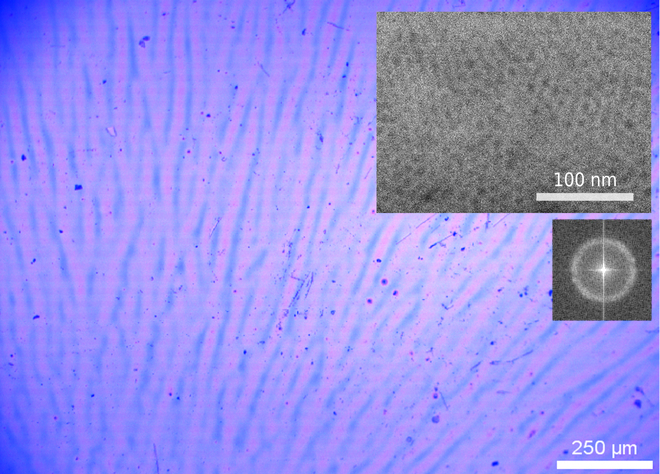
\includegraphics[width=\textwidth]{Imagenes/Si_BF127-Combinada.jpg}
	   		\end{subfigure}
			 \caption[Microscopía óptica \pdmF tratamiento en medio básico.]{Microscopías ópticas para \pdmF\space sintetizadas por el tratamiento de condensación y extracción en medio básico. Izquierda: sobre sustrato de Au. Derecha: sobre sustrato de Si.}
			 \label{fig:Microscopia_F127_basico}	
		     \end{figure}	
		
		En las elipsoporosimetría realizadas para el sistema \pdmF\space se vuelve a observa la <<doble distribución>> muy similar a la obtenida por el tratamientos en medio ácido, pero en este caso el índice de refracción es $n=1.22$ el cual es prácticamente idéntico al de un sistema calcinado (figura \ref{fig:F127_basico_EPA} ).

		\begin{figure}[!ht]
		  	\begin{subfigure}[t]{0.495\textwidth}
		  	\includegraphics[width=\textwidth]{Graficos/SI_F127_basico_EPA.pdf}
			\caption[Elipsoporsimetría \pdmF\space tratamiento básico.]{Isoterma de adsorción/desorción de agua realizada por PEA para una \pdmF.}
			\label{fig:F127_basico_EPA}
			\end{subfigure}
			\begin{subfigure}[t]{0.495\textwidth}
		  	\includegraphics[width=\textwidth]{Graficos/SI_F127_basico_PSD.pdf}
			\caption{Distribución de tamaño de poro y cuello.\\ }
			\label{fig:F127_basico_PSD}
			\end{subfigure}
			\caption[Elipsoporosimetría \pdmF\space tratamiento básico.]{Resultados de elipsoporosimetría ambiental para una \pdmF\space sintetizada por el tratamiento en medio básico.}
			\end{figure}

		El sistema sintetizado en medio básico usando CTAB como surfactante muestra una película muy fraccionada cuando el sustrato es Au y una película homogéneamente depositada cuando es silicio, como se puede apreciar en las microscopías de la figura \ref{fig:Microscopia_CTAB_basico}. Los resultados de las mediciones por PEA muestran un sistema con muy porosos ($40\%$) y un índice de refracción $n=1,22$.
			
		\begin{figure}[!th]
 	   	    \begin{subfigure}[t]{0.49\textwidth}
	       	\includegraphics[width=\textwidth]{Imagenes/Au_BCTAB-Combinada.jpg}
	   		\end{subfigure}
	   		\begin{subfigure}[t]{0.49\textwidth}
	   	    \includegraphics[width=\textwidth]{Imagenes/Si_BCTAB-Combinada.jpg}
	   		\end{subfigure}
			 \caption[Microscopía óptica \pdmC tratamiento en medio básico.]{Microscopías ópticas para \pdmC\space sintetizadas por el tratamiento de condensación y extracción en medio básico. Izquierda: sobre sustrato de Au. Derecha: sobre sustrato de Si.}
			 \label{fig:Microscopia_CTAB_basico}	
		     \end{figure}		

		\begin{figure}[!ht]
		  	\begin{subfigure}[t]{0.495\textwidth}
		  	\includegraphics[width=\textwidth]{Graficos/SI_CTAB_basico_EPA.pdf}
			\caption[Elipsoporsimetría \pdmC\space tratamiento básico.]{Isoterma de adosroción/desorción de agua realizada por PEA para una \pdmC.}
			\label{fig:CTAB_basico_EPA}
			\end{subfigure}
			\begin{subfigure}[t]{0.495\textwidth}
		  	\includegraphics[width=\textwidth]{Graficos/SI_CTAB_basico_PSD.pdf}
			\caption{Distribución de tamaño de poro y cuello.\\ }
			\label{fig:CTAB_basico_PSD}
			\end{subfigure}
			\caption[Elipsoporosimetría \pdmC\space tratamiento básico.]{Resultados de elipsoporosimetría ambiental para una \pdmC\space sintetizada por el tratamiento en medio básico.}
			\end{figure}

		En el IR para ambos surfactantes (figura \ref{fig:IR_CTAB_basico} para CTAB y \ref{fig:IR_F127_basico} para F127) se observa una ruptura del típico hombro para estructuras mesoporososas de sílice\cite{Olsen1989,Innocenzi2003,Angelome2008}, (presente a mayores frecuencias de TO$_3$) indicando un posible colapso de la organización de poros en la nanoescala, posiblemente debido a la disolución parcial de la sílice, dada por el medio básico. Si bien el medio básico cataliza la hidrólisis del TEOS, también aumenta la tasa de disolución del SiO$_2$.\cite{Mazer1994,Niibori2000,Gorrepati2010}

		\begin{figure}[!ht]
			\begin{center}
			\includegraphics[width=0.75\textwidth]{Graficos/IR_F127_basico.pdf}
			\caption[FTIR \pdmF\space tratamiento básico.]{Espectro de absorción en el IR para una \pdmF\space sintetizada con el tratamiento básico antes y después de extraer el surfactante. Obsérvese la ausencia de hombro en la región 1250-\SI{1100}{\cm^{-1}}, la cual es típica de sistemas de SiO$_2$ mesoestrucuturas.}
			\label{fig:IR_F127_basico}
			\end{center}
			\end{figure}

        \clearpage

		\begin{figure}[!ht]
			\begin{center}
			\includegraphics[width=0.75\textwidth]{Graficos/IR_CTAB_basico.pdf}
			\caption[FTIR \pdmC\space tratamiento básico.]{Espectro de absorción en el IR para una \pdmC\space sintetizada con el tratamiento básico antes y después de extraer el surfactante. Obsérvese la ausencia de hombro en la región 1250-\SI{1100}{\cm^{-1}}, la cual es típica de sistemas de SiO$_2$ mesoestrucuturas.}
			\label{fig:IR_CTAB_basico}
			\end{center}
			\end{figure}		

\section{Discusión sobre los distintos tratamientos}

		Luego de depositar, sintetizar, llevar a cabo los tratamientos y caracterizar las distintas películas, se hace aquí, una discusión de los resultados sobre cada sistema. El resultado de la discusión y el análisis llevará a elegir uno o más tratamientos adecuados para la fabricación de los sensores basados en películas mesoporosas.
 		
 	\subsection{Sobre los sustratos}
	
		Es importante destacar que el objetivo es depositar las películas mesoporosas sobre un sustrato óptimo para hacer reacciones electroquímicas. En este caso se elijó el Au. Sin embargo, para llevar a cabo numerosas caracterizaciones, entender las bases de algunos comportamientos y comparar con la literatura, fue necesario hacer algunos depósitos sobre silicio.

		Los sistemas que usaron CTAB y fueron depositados sobre Au presentaron todos grietas, fracturas y discontinuidades, como se mencionó en el capitulo anterior esto es producto de la adsorción superficial del Br sobre el Au. 

		Hubo dos tratamientos en particular, el tratamientos en medio ácido y el tratamiento en medio básico, que mostraron el mismo comportamiento independientemente del surfactante utilizado estructurar el óxido. Ambos presentan grietas a lo largo de toda la película sobre sustrato de Au. Esto es resultado de dos factores combinados, la baja adherencia sobre sustrato de Au (a los sistemas con CTAB se le suma la adsorción del surfactante al sustrato) y la violenta condensación en cada medio debido al tratamiento, esto lleva a una contracción en todas direcciones, generando las grietas, ya que la fuerza de adherencia al Au no es suficiente para aguantar la contracción en el plano de la películas. No pasó lo mismo cuando el sustrato es silicio donde la contracción (como es lo habitual para sistemas calcinados) ocurre solo en el eje normal a la película.

		El resto de los tratamientos sobre Au para F127 resultaron homogéneamente depositados.

		Respecto de la adherencia sobre silicio, todos lo tratamientos fueron exitosos para ambos surfactantes.

    \subsection{Sobre la condensación}	
	
	 	Una de las dos técnicas que uso para evaluar la condensación de las películas fue la espectroscopia IR.	

		 \begin{table}[!ht]
			\caption[Resumen FTIR para tratamientos alternativos]{Resumen del análisis por FTIR para los distintos tratamientos pos-depósito aplicados a las películas nanoporosas de SiO$_2$. Los valores corresponden a la relación Si-O-Si/Si-OH.}
			
			\begin{tabular}{>{\raggedright\arraybackslash}m{3cm}>{\raggedright\arraybackslash}m{0.25cm}>{\centering\arraybackslash}m{0.8cm}>{\centering\arraybackslash}m{2cm}>{\raggedright\arraybackslash}m{0.3cm}>{\centering\arraybackslash}m{0.8cm}>{\raggedright\arraybackslash}m{2cm}}
			\toprule

			 Sistema$^*$ & & \multicolumn{2}{c}{Sin extraer} &  & \multicolumn{2}{c}{Extraído} \\

			\midrule
		 
			 CTAB Calcinado 	& & $-$	   & 		$-$	   & & $1.077$    & Hombro LO$_3^\dagger$ \\
			 CTAB Simplificado  & & $0.30$ & TO$_4-$LO$_4^\mathsection$ & & $	0.67$  & Hombro LO$_3$ \\
			 CTAB Prolongado 	& & $0.27$ & TO$_4-$LO$_4$ & & $0.80$     & Hombro LO$_3$ \\
			 CTAB Alto vacío 	& & $0.38$ & TO$_4-$LO$_4$ & & $0.88$     & Hombro LO$_3$ \\
			 CTAB Ácido 		& & $0.33$ & TO$_4-$LO$_4$ & & $0.80$     & Hombro LO$_3$ \\
			 CTAB Básico 		& & $0.33$ & TO$_4-$LO$_4$ & & $0.99$	  & TO$_4-$LO$_4$ \\

			\midrule

			 F127 Calcinado 	& & 	$-$ 	 & 		$-$	   & & $0.77$    & Hombro LO$_3$ \\
			 F127 Simplificado  & & $0.24$ & Hombro LO$_3$ & & $0.53$   	      & Hombro LO$_3$ \\
			 F127 Prolongado 	& & $0.32$ & Hombro LO$_3$ & & $0.78 $   & Hombro LO$_3$ \\
			 F127 Alto vacío 	& & $0.27$ & Hombro LO$_3$ & & $0.78 $   & Hombro LO$_3$ \\
			 F127 Ácido 		& & $0.30$ & Hombro LO$_3$ & & $0.80 $   & Hombro LO$_3$ \\
			 F127 Básico 		& & $0.28$ & Hombro LO$_3$ & & $0.99$		      & TO$_4-$LO$_4$ \\
			
			\bottomrule
			\end{tabular}\vspace*{2pt}
			\footnotesize{$^*$Todos los tratamientos sobre sustrato de Si tratado previamente con HF.}\\
			\footnotesize{$^\dagger$ Se refiere a la banda típica para sistemas mesoporosoros de SiO$_2$.} \\
			\footnotesize{$^\mathsection$Se refiere al acoplamiento TO$_4-$LO$_4$ presente en sistemas desordenados.}
			\label{tabla:Resultados_IR}
			\end{table}
	
			Siguiendo la relación de picos Si-O-Si/Si-OH se puede evaluar el grado de condensación de la red de óxido de silicio. Un número más grande indica mayor cantidad de enlaces Si-O-Si, por lo tanto mayor grado de condensación. Otra banda importante es el hombro de LO$_3$ formado a mayores frecuencia de TO$_3$ característico de estructuras porosas de SiO$_2$. La ausencia de este hombro o predominancia de la frecuencia del fonon compuesto por las vibraciones TO$_4$-LO$_4$ es indicador de un sistema desordenado\cite{Innocenzi2003,Lange1990,Lange1989}, lo que le atribuimos, junto a otros indicios al colapso de la estructura porosa. En la tabla \ref{tabla:Resultados_IR} se muestras los valores cuantitativos respecto de estas bandas.

			La otra técnica fue la elipsoporosimetria ambiental (PEA). De esta técnica podemos extraer datos como el índice de refracción del SiO$_2$ poroso ponderando su porosidad, según la aproximación de Bruggeman\cite{Bruggeman1935}. Este valor, comparado con el sistema calcinado, nos da una idea de cuan condensada esta la película. También extraemos de las isotermas la porosidad, tamaño de poro y cuello. Todos los sistemas resultaron porosos, sin embargo para el F127, muchos de los tratamientos (simplificado, ácido y básico) presentaron doble distribución de cuellos. 

			\begin{figure}[!th]
		 	   	    \begin{subfigure}[t]{0.49\textwidth}
			       	\includegraphics[width=\textwidth]{Graficos/SI_CTAB_todos_EPA.pdf}
			   		\end{subfigure}
			   		\begin{subfigure}[t]{0.49\textwidth}
			   	    \includegraphics[width=\textwidth]{Graficos/SI_F127_todos_EPA.pdf}
			   		\end{subfigure}
					 \caption[Comparación PEA tratamientos alternativos]{Comparación de las elipsoporosimetría ambientales para todos los tratamientos experimentados. Izquieda: resultados cuando se estructuran con CTAB, notesé los altos índices de refracción para los tratamientos simplicado y en medio ácido. Drecha: resultados cuando se estructuran con F127, donde se destacan las <<doble distribuciones>> de cuellos y poros.}
					 \label{fig:todos_EPA}	
				     \end{figure}


			Para todos los tratamientos los índices de refracción dan valores comparables con óxidos mesoporosos calcinados, indicando una condensación similar a estos. En las figura \ref{fig:todos_EPA} se comparan todas las isotermas para cada uno de los sistemas, estructurado con CTAB y con F127. En la tabla \ref{tabla:Resultados_EPA} se resumen los datos extraídos de las isotermas de adsorción/desorción de agua.
	
			\begin{table}[ht]
				\caption[Resumen PEA para tratamientos alternativos]{Resumen del análisis por PEA para los sistemas estructurados con CTAB y F127 de los distintos tratamientos pos-depósito aplicados a las películas nanoporosas de SiO$_2$.}
				\begin{tabular}{>{\raggedright\arraybackslash}m{3cm}>{\centering\arraybackslash}m{2.2cm}>{\centering\arraybackslash}m{2cm}>{\centering\arraybackslash}m{2cm}>{\centering\arraybackslash}m{0.8cm}}
				\toprule

				 Sistema$^*$ &  Porosidad(\%) & Diámetro Poro (nm)   & Diámetro Cuello (nm) & $n^\dagger$ \\

				\midrule

				 CTAB Calcinado 	& $44$ & $2.5$ & $2.0$ & $1.384$ \\
				 CTAB Simplificado  & $30$ & $2.2$ & $2.0$ & $1.389$ \\
				 CTAB Prolongado 	& $41$ & $2.4$ & $1.2$ & $1.375$ \\
				 CTAB Alto vacío 	& $44$ & $2.0$ & $1.6$ & $1.393$ \\
				 CTAB Ácido 		& $39$ & $2.0$ & $1.5$ & $1.386$ \\
				 CTAB Básico 		& $46$ & $2.3$ & $1.6$ & $1.396$ \\
				\midrule

				 F127 Calcinado 	& $38$ & $10.2$ & $4.4$ & $1.390$ \\
				 F127 Simplificado$^\mathsection$  & $30$ & $8.0$  & $ - $ & $1.390$ \\
				 F127 Prolongado$^\mathsection$ 	& $39$ & $7.8$ & $ - $ 	& $1.381$ \\
				 F127 Alto vacío 	& $28$ & $9.0$ & $3.5$  & $1.383$ \\
				 F127 Ácido$^\mathsection$ 		& $30$ & $5.4$ & $ - $  & $1.399$ \\
				 F127 Básico$^\mathsection$ 		& $34$ & $6.8$ & $ - $  & $1.374$ \\
				\bottomrule
				\end{tabular}\vspace*{2pt}
				\footnotesize{$^*$Todos los tratamientos sobre sustrato de Si tratado previamente con HF.}\\
				\footnotesize{$^\dagger$Los valores corresponden al $n$ calculado para las paredes de los sistemas mesoporosos.}\\
				\footnotesize{$^\mathsection$Sistemas con doble distribución de cuello.} \\
				\label{tabla:Resultados_EPA}
				\end{table}	
		
    \subsection{Sobre la extracción}	
		
		Las extracciones en todos los caso fueron llevadas a cabo en un reflujo de 2-propanol. Si bien fueron exitosa en todos los casos siempre queda una pequeña banda que se observa en el IR. Esta banda corresponde a la vibración C-H, y puede provenir tanto del surfactante como de un intercambio del hidroxilo por el propanol, tal como se muestra en la siguiente ecuación:
			\begin{equation}
				 \schemestart 
				 Si-OH + OH-CH$_2$CH$_3$ 
				 \arrow{<=>}[0,1.5] 
				 Si-O-CH$_2$CH$_3$ + H$_2$O
				 \schemestop
				 \label{eq:prolilo}
				 \end{equation}
		Por este motivo, luego de la extracción con 2-propanol, se realizó un enjuague sobre las muestras con H$_2$O ligeramente acidificada con HCl (pH$\approx 2$), de forma de no afectar al óxido, y poder terminar de extraer residuos de surfactante o propanol ligado a la estructura. En la figura \ref{fig:IR_agua} se muestra el resultado de este enjuague en un sistemas sílice F127 preparado por el método de alto vacío.

			\begin{figure}[!ht]
			\begin{center}
			\includegraphics[width=0.75\textwidth]{Graficos/IR_F127_vacio_AGUA.pdf}
			\caption[FTIR extracción agua ácida.]{Espectro de absorción de IR correspondiente a una \pdmF\space sintetizada por el tratamiento prolongado en vacío antes de la extracción, después de la extracción con 2-propanol y tratamiento enjuague posterior con agua ácida.}
			\label{fig:IR_agua}
			\end{center}
			\end{figure}

\section{Conclusiones parciales}

	En este capitulo, se volcaron los resultados de un trabajo sistemático y metódico sobre los procesos de síntesis a bajas temperaturas de películas de óxido de silicio mesoporosos, estructuradas con Pluronic F127 y bromuro de hexadeciltrimetilamonio (CTAB). El esquema de la figura \ref{fig:modelo-problemas} sintetiza los problemas a superar durante el proceso de síntesis de las películas.

			\begin{figure}[!ht]
			\begin{center}
			\includegraphics[width=0.75\textwidth]{Esquemas/esquema-problemas.pdf}
			\caption[Modelo de los problemas tecnologicos]{Esquema en sección transversal de los sensores y los problemas tecnológicos asociados cuando se combinan los procesos\textit{ bottom-up} y\textit{ top-down}. \unorojo Falta de adherencia entre las \pdm\space y el Au. \dosvioleta Bloqueo de los electrodos para realizar reacciones redox debido a la difusión desde las capas metálicas a la interfaz electrodo\textbar mesoporoso. \tresamarillo Desarrollo de un método de síntesis a baja temperatura para minimizar los efectos difusivos. \cuatronaranja Extraer los remanentes de surfactante dentro de los poros ya que las películas no son sometidas a temperaturas de calcinación.}
			\label{fig:modelo-problemas}
			\end{center}
			\end{figure}
	

	Los resultados muestran que cualquiera de los métodos es plausible de ser usado para obtener \pdm, con poros accesibles, y porosidades entre 30 y 45\% aproximadamente. Sin embargo, este trabajo busca poder utilizar estas películas como elemento activo permeoselectivo incorporado en sensores electroactivos. Para ello no basta solo con obtener películas mesoporosas sobre silicio o vidrio (sistemas mas clásicos), sino que hay que sintetizarlas sobre electrodos de buena respuesta electroquímica, como el Au o Pt, para llevar a cabo la detección de los analitos. También es preciso mantener, durante todo el proceso de síntesis, la temperatura por debajo de los \SI{150}{\celsius} para evitar procesos difusivos, como explicaremos en los próximos capítulos.

	Las películas estructuras con F127 mostraron dificultades a la hora de obtener distribuciones homogéneas de poro y cuello. Los tratamientos simplificado, prolongado, ácido y básico mostraron estos inconvenientes, sin embargo con tiempo prologando en vacío las películas resultaron homogéneas en todo sentido, tanto en el deposito en sí, como en un única distribución de cuello y poro. 

	No fue posible obtener depósitos continuos sobre Au en películas estructuras con CTAB. Esto se debe a las limitaciones de adherencia sobre Au (que fueron explicados en el capítulos anterior), sumado a la adsorción del CTAB sobre la superficie del mismo. A pesar de ello, los métodos desarrollados sobre silicio demostraron ser parcialmente exitosos en todos los casos.

	De los 5 métodos desarrollados, solo el de alto vacío resulto ser apto para utilizar indistintamente CTAB o F127. Tampoco mostró problemas de adherencia sobre Au cuando se estructuro con F127. Este resultado resulta interesante en sí, ya que, si bien las películas con CTAB sobre Au no adhieren, es importante saber que el proceso de síntesis es compatible con este tipo de películas, ya que permitiría combinar dispositivos multicapas mixtos de CTAB y/o F127 en un solo proceso de síntesis.

	Por supuesto el tema principal es que, a diferencia de los métodos existentes hasta ahora, en ninguno de los procesos la temperatura se eleva mas de \SI{130}{\celsius}. Evitar la calcinación permite trabajar sobre sustratos térmicamente lábiles, como polímeros, y evitar procesos difusivos en las interfaces electrodos-mesoporoso. 

	Si se piensa en sensores y procesos de fabricación complejos, que involucren algunas etapas de fabricación, se podría usar cualquiera de los métodos desarrollados, eligiendo adecuadamente según el propósito que se persigue. Por ejemplo, si se desea funcionalizar las películas con polímeros o si se usan sustratos químicamente más lábiles, hay que tener en cuenta que de los métodos en medios ácidos o básicos son químicamente muy agresivos, pero son rápidos y económicos.

	El tema central de los próximos dos capítulos es el estudio de los fenómenos de transporte de sondas electroquímicas a través de películas mesoporosos sobre electrodos de Au microfabricados. Para estudiar dichos fenómenos se fabricaron sensores prototipos en base a películas mesoporosas de SiO$_2$ estructuradas con F127 y sintetizadas por el método de alto vacío. Se eligió este método porque es el mas suave desde el el punto de vista químico, el mas compatible con otras películas mesoporosas y el que resultó tener buena adherencia con el Au.	

	Por último se resumen en el diagrama de la figura \ref{fig:flujo-trabajo} el flujo de trabajo para el desarrollo de películas mesoporosas de óxido de silicio a bajas temperaturas.

	\begin{figure}[!ht]
			\begin{center}
			\includegraphics[width=0.75\textwidth]{Esquemas/arbol-problemas.pdf}
			\caption[Flujo de trabajo para obtener electrodos con películas mesoporosa]{Diagrama árbol donde se muestra las etapas y tratamientos utilizadas con sus problemas asociados, para lograr fabricar electrodos recubiertos con películas delgadas meosoporosas de óxido de silicio}
			\label{fig:flujo-trabajo}
			\end{center}
			\end{figure}		

%Poner al final de este capitulo un apartado con informacion suplementaria o hacer un anexo al final de la tesis que diga Anexo: Infomarmacion suplementaria: EN este anexo se agregan todos los graficos que no se colocaron en el cuerpo del texto para hacer la lectura mas fluida.